Ce projet de C a été très enrichissant d'un point de vue travail de groupe, organisationnel et intellectuel. Étant le premier projet a réaliser à quatre sur notre temps personnel, cela n'a pas été facile de joindre nos emplois du temps. Ce projet s'est finalement très bien déroulé. Lors de nombreuses réunions, le travail a été défini, expliqué et réparti, selon nos forces et nos faiblesses. De plus, nous avons pu mettre en application et développer toutes les connaissances vues en Langage C, Méthodologie Conception Logicielle et même Architectures des calculateurs. Pour finir, ce projet nous laisse encore de grandes possibilités d'évolutions comme par exemple le codage de l'APU, de l'IHM, le développement de nouveaux mappers et la mise en place de fonctions telles que la sauvegarde. Nous estimons un total d'environ cinq à six mois pour coder l'intégralité de ces fonctions. Il faudrait un mois pour l'APU ainsi qu'un autre pour l'IHM. Le développement des mappers serait plus long. En effet, il s'agirait de rendre notre émulateur capable de lire quatre à cinq autres types de cartouches NES. Cela permettrait de pouvoir jouer à une grande majorité des jeux. De plus, l'émulateur demande beaucoup de ressources au processeur. Il est difficile de tenir les 60 FPS sur certaines machines. Il serait donc nécessaire de l'optimiser avec une technique de prédiction, c'est à dire émuler un composant à un moment $t$ que si celui-ci a été ciblé par le programme en exécution sur le 6502.

\begin{figure}[H]
  \centering
   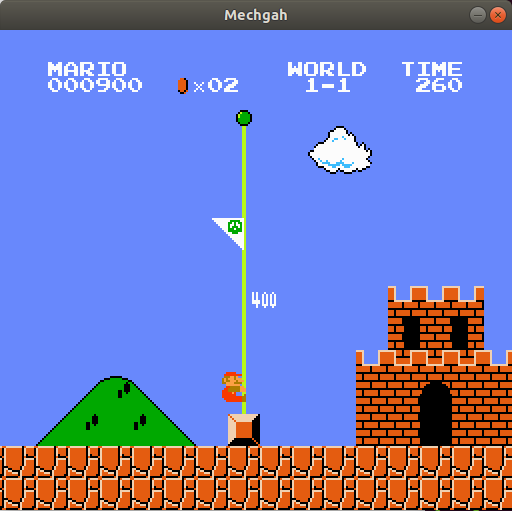
\includegraphics[width=0.50\linewidth]{images/smb_nes.png}
   \caption{Capture d'écran de l'émulateur sur le jeu \emph{Super Mario Bros}}
   \label{fig:gantt_fin}
\end{figure}
